\documentclass[aspectratio=169,11pt]{beamer}

% ============================================================
% PACKAGES
% ============================================================
\usepackage{graphicx}
\usepackage{underscore}
\usepackage{tikz}
\usetikzlibrary{positioning,arrows.meta}
\usepackage{xcolor}
\usepackage{booktabs}
\usepackage{tabularx}
\usepackage{array}
\usepackage{ragged2e}
\usepackage{hyperref}

% ============================================================
% COLORS - SAME AS PHASE-I
% ============================================================
\definecolor{GEUBlue}{RGB}{20,55,105}
\definecolor{GEULightBlue}{RGB}{238,244,251}
\definecolor{GEUGrey}{RGB}{90,90,90}
\definecolor{GEULightGrey}{RGB}{245,246,248}

% ============================================================
% BEAMER SETTINGS
% ============================================================
\usetheme{default}
\setbeamertemplate{navigation symbols}{}
\setbeamertemplate{blocks}[rounded][shadow=false]

\setbeamercolor{normal text}{fg=black,bg=white}
\setbeamercolor{frametitle}{fg=GEUBlue}
\setbeamercolor{structure}{fg=GEUBlue}
\setbeamercolor{block title}{fg=GEUBlue,bg=GEULightBlue}
\setbeamercolor{block body}{fg=black,bg=GEULightBlue}

\setbeamerfont{frametitle}{size=\Large,series=\bfseries}

% ============================================================
% LOGO
% ============================================================
% Upload the Graphic Era logo with this filename to Overleaf.
\newcommand{\GEULogo}{graphicera_logo.png}

% ============================================================
% HEADER
% ============================================================
\setbeamertemplate{headline}{%
  \begin{tikzpicture}[remember picture,overlay]
    \node[
        anchor=north east,
        xshift=-0.30cm,
        yshift=-0.12cm
    ] at (current page.north east)
    {\includegraphics[height=0.62cm]{\GEULogo}};
  \end{tikzpicture}
  \vspace{0.72cm}
}

% ============================================================
% FRAME TITLE
% ============================================================
\setbeamertemplate{frametitle}{%
  \vspace{0.03cm}
  \insertframetitle\par
  \vspace{0.04cm}
  \textcolor{GEUBlue}{\rule{\textwidth}{0.9pt}}
  \vspace{0.03cm}
}

% ============================================================
% FOOTER
% ============================================================
\setbeamertemplate{footline}{%
  \leavevmode
  \hbox{%
  \begin{beamercolorbox}[
      wd=.82\paperwidth,
      ht=0.32cm,
      dp=0.10cm,
      leftskip=.3cm
  ]{author in head/foot}
    \tiny Department of Computer Science \& Engineering |
    Graphic Era (Deemed to be University)
  \end{beamercolorbox}%
  \begin{beamercolorbox}[
      wd=.18\paperwidth,
      ht=0.32cm,
      dp=0.10cm,
      rightskip=.3cm
  ]{date in head/foot}
    \hfill\tiny\insertframenumber/\inserttotalframenumber
  \end{beamercolorbox}}
}

% ============================================================
% CUSTOM COMMANDS
% ============================================================
\newcommand{\smallnote}[1]{%
\vspace{0.08cm}
{\scriptsize\color{GEUGrey}#1}
}

\newcommand{\placeholder}[1]{%
\textit{\color{GEUGrey}#1}
}

% ============================================================
% DOCUMENT INFORMATION
% ============================================================
\title{\textbf{Project-Based Learning}\\[2mm]\large Phase-II Evaluation}
\author{\textbf{Project Title}\\Team ID: XXXX}

\institute{
Department of Computer Science \& Engineering\\
Graphic Era (Deemed to be University), Dehradun
}

\date{Academic Session 2026--27}

% ============================================================
% DOCUMENT
% ============================================================
\begin{document}

% ============================================================
% SLIDE 1
% ============================================================
\begin{frame}[plain]

\begin{tikzpicture}[remember picture,overlay]

\draw[GEUBlue,line width=3pt]
(current page.north west) -- (current page.north east);

\node[
    anchor=north east,
    xshift=-0.45cm,
    yshift=-0.35cm
] at (current page.north east)
{\includegraphics[height=1.0cm]{\GEULogo}};

\node[
    align=center,
    text width=.84\paperwidth
] at ([yshift=.25cm]current page.center)
{
{\color{GEUBlue}
\fontsize{26}{30}\selectfont
\bfseries PROJECT-BASED LEARNING}
\\[3mm]

{\fontsize{18}{22}\selectfont
PHASE-II EVALUATION}
\\[7mm]

{\color{GEUGrey}
\Large\bfseries
\placeholder{STUDYWISE: STUDY MATERIAL \\ORGANISING AND SMART PLANNING SYSTEM}}
\\[3mm]

{\color{GEUBlue}
\normalsize Team ID: DSCPP-III-2026-T304}
};

\node[
    align=center,
    anchor=south,
    yshift=.42cm
] at (current page.south)
{
\bfseries
Department of Computer Science \& Engineering\\
Graphic Era (Deemed to be University), Dehradun\\[-1mm]
\scriptsize Academic Session 2026--27
};

\end{tikzpicture}

\end{frame}

% ============================================================
% SLIDE 2
% ============================================================
\begin{frame}{Team \& Mentor Details}

\begin{columns}[T,totalwidth=\textwidth]

\column{.48\textwidth}

\begin{block}{Team Information}
\begin{tabular}{@{}ll@{}}
\textbf{Team ID:} & DSCPP-III-2026-T304\\
\textbf{Semester:} & 3rd\\
\textbf{Section:} & C,F,K\\
\end{tabular}
\end{block}

\column{.48\textwidth}

\begin{block}{Team Members}
1.\quad \placeholder{REHMAN ULLAH KHAN -- 2510012769}\\
2.\quad \placeholder{MANAN LOHNI -- 2510012770}\\
3.\quad \placeholder{DIPANSHU SIROHI -- 2510360064}\\
\end{block}

\end{columns}

\vspace{2mm}

\begin{block}{Mentor}
\placeholder{ Ms. Megha Garg}
\hfill
\textbf{Interactions completed:}
\underline{   6\hspace{12mm}}
\end{block}

\vfill

\end{frame}

% ============================================================
% SLIDE 3
% ============================================================
\begin{frame}{Phase-I Recap \& Feedback Incorporated}
\vspace{-6mm}
\begin{block}{Phase-I Status}
\placeholder{1.Identified the problem of organizing study materials and deciding which topics to study first.\\
2.Defined the project objectives and proposed the STUDYWISE solution.\\
3.Identified the planned use of C++, OOP concepts, DSA, and file handling.\\
4.Outlined the major modules, expected features, and development milestones for Phase II.
}
\end{block}

\vspace{0.1mm}

\begin{columns}[T,totalwidth=\textwidth]

\column{.48\textwidth}

\textbf{\color{GEUBlue}Feedback Received}

\begin{itemize}\itemsep2pt
\item \placeholder{Clarify how study materials will be organized.}
\item \placeholder{Define the factors used for topic priority calculation.}

\end{itemize}

\column{.48\textwidth}

\textbf{\color{GEUBlue}Changes Incorporated}

\begin{itemize}\itemsep2pt
\item \placeholder{Identified priority factors such as exam urgency, difficulty, and remaining syllabus.}


\item \placeholder{Improved the proposed approach for subject-wise study material organization.}
\end{itemize}

\end{columns}

\vfill



\end{frame}

% ============================================================
% SLIDE 4
% ============================================================
\begin{frame}{Problem Statement \& Finalized Objectives}
\vspace{-6mm}
\begin{block}{Problem Statement}
\placeholder{Students often struggle to organize their academic subjects and study resources and decide which topics require attention first. STUDYWISE aims to address these challenges through a C++-based system that manages academic records, applies searching and sorting algorithms, and prioritizes unfinished topics according to exam urgency and academic factors.}


\end{block}

\vspace{1mm}

\textbf{\color{GEUBlue}Finalized Objectives}

\begin{enumerate}\itemsep3pt
\item \placeholder{Manage academic subjects and topics using C++ classes and objects.}
\item \placeholder{Implement searching and sorting algorithms for efficient record retrieval.}
\item \placeholder{Calculate topic priorities using academic factors and a custom Max Heap.}
\item \placeholder{Extend the system in Phase III with study-material organization and daily study planning.}
\end{enumerate}

\vfill



\end{frame}

% ============================================================
% SLIDE 5
% ============================================================
\vspace{-5cm}
\begin{frame}{Updated System Architecture / Workflow}
\vspace{-0.8cm}
\begin{left}

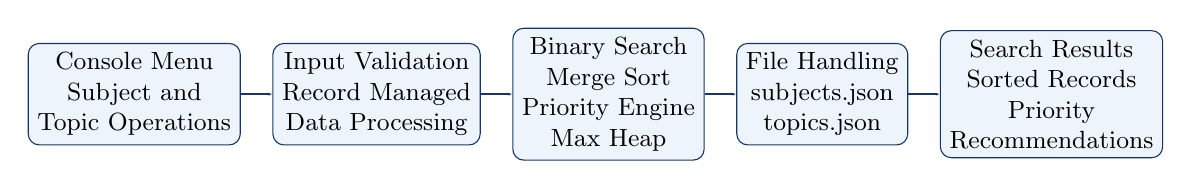
\begin{tikzpicture}[
node distance=4mm,
box/.style={
rectangle,
rounded corners,
draw=GEUBlue,
fill=GEULightBlue,
minimum width=1.5cm,
minimum height=5mm,
align=center,
font=\small
},
arrow/.style={
-{Latex[length=0.5mm]},
thick,
draw=GEUBlue
}
]

\node[box] (a) {Console Menu\\Subject and\\Topic Operations};
\node[box,right=of a] (b) {Input Validation\\Record Managed\\Data Processing};
\node[box,right=of b] (c) {Binary Search\\Merge Sort\\Priority Engine\\Max Heap};
\node[box,right=of c] (d) {File Handling\\subjects.json\\topics.json};
\node[box,right=of d] (e) {Search Results \\Sorted Records \\Priority\\ Recommendations};

\draw[arrow] (a)--(b);
\draw[arrow] (b)--(c);
\draw[arrow] (c)--(d);
\draw[arrow] (d)--(e);

\end{tikzpicture}

\end{center}

\vspace{0.2cm}

\begin{columns}[T,totalwidth=\textwidth]

\column{.48\textwidth}

\textbf{\color{GEUBlue}Major Components}

\begin{itemize}\itemsep2pt
\item \placeholder{Subject and Topic Management.}\\\\
\vspace{2mm}
\item \placeholder{Searching and Sorting Engine.}
\vspace{2mm}
\item \placeholder{Priority Recommendation Engine.}
\vspace{2mm}
\item \placeholder{File Handling and JSON Persistence.}
\vspace{2mm}
\end{itemize}

\column{.48\textwidth}

\textbf{\color{GEUBlue}Changes Since Phase-I}

\begin{itemize}\itemsep2pt
\item \placeholder{Implemented subject and topic management using OOP concepts.}
\item \placeholder{Added searching, sorting, and priority-based recommendation logic.}
\item \placeholder{Prepared a separate frontend visual prototype for planned Phase III integration.}
\end{itemize}

\end{columns}

\vfill


\end{frame}

% ============================================================
% SLIDE 6
% ============================================================
\begin{frame}{Module Design \& Functional Requirements}

\begin{columns}[T,totalwidth=\textwidth]

\column{.48\textwidth}
\vspace{-0.7cm}
\textbf{\color{GEUBlue}Major Modules}

\begin{enumerate}\itemsep3pt
\item \placeholder{Manages academic records,and subject-topic relationships.}
\item \placeholder{Implements Linear Search, Binary Search, and Merge Sort to retrieve and organize records.}
\item \placeholder{The system shall calculate topic priority scores and recommend unfinished topics in priority order.}
\item \placeholder{Loads and saves subject and topic records to maintain data between program executions.}
\end{enumerate}

\column{.48\textwidth}
\vspace{-0.7cm}


\textbf{\color{GEUBlue}Functional Requirements}

\begin{itemize}\itemsep3pt
\item \placeholder{The system shall allow users to create, view, update, and delete subject and topic records.}
\item \placeholder{The system shall search for records and sort them using the implemented algorithms.}
\item \placeholder{The system shall calculate topic priority scores and recommend unfinished topics in priority order.}
\item \placeholder{The system validate input data and persist subject and topic records using file handling.}
\end{itemize}

\end{columns}

\vfill

\begin{block}{Module Dependency}
\placeholder{
Briefly describe dependencies and interactions between major modules.
}
\end{block}

\smallnote{
Brief Discussion: Explain what each module does and how it contributes
to the complete system.
}

\end{frame}

% ============================================================
% SLIDE 7
% ============================================================
\begin{frame}{Technology Stack \& Development Methodology}

\begin{columns}[T,totalwidth=\textwidth]

\column{.48\textwidth}
\vspace{-0.5cm}
\begin{block}{Technology Stack}

\begin{itemize}\itemsep2pt
\item Programming: \placeholder{ C++ }
\item Framework : \placeholder{Console-based Cpp}
\item Compiler: \placeholder{MinGW GCC 6.3.0}
\item Development Tool: \placeholder{VS Code}
\item Data Persistence: \placeholder{File handling}
\item Frontend Prototype: \placeholder{React.js and Vite}
\item Version Control: \placeholder{GitHub}
\end{itemize}

\end{block}

\column{.48\textwidth}
\vspace{-0.5cm}

\begin{block}{Development Methodology}

\begin{enumerate}\itemsep2pt
\item Identified student study management problems and defined project objectives.
\item Planned modules, class structures, algorithms, and data flow.
\item Developed C++ OOP classes, searching and sorting algorithms, and the priority engine.
\item Connected backend modules and implemented JSON-based persistence.
\end{enumerate}

\end{block}

\end{columns}

\vfill


\end{frame}

% ============================================================
% SLIDE 8
% ============================================================
\begin{frame}{Implementation of PBL Course Concepts}

\scriptsize

\begin{center}

\renewcommand{\arraystretch}{1.25}

\begin{tabularx}{.96\textwidth}
{@{}>{\bfseries}p{3.0cm}X p{2.5cm}@{}}

\toprule
Course/Area & Concepts Actually Implemented & Project Module\\
\midrule

Data Structures in C &
\placeholder{Linear Search, Binary Search, Merge Sort, custom Max Heap} &
\placeholder{SearchSortEngine.cpp PriorityEngine.cpp}\\

OOPs with C++ &
\placeholder{Classes, Objects,STL,Encapsulation, Constructors, Data Validation} &
\placeholder{Subject and Topic models, Manager classes}\\

File Handling &
\placeholder{File streams, fstream , serialization,data storage} &
\placeholder{Subject and Topic Managers}\\

Algorithm Design &
\placeholder{Weighted Priority Calculation, Heap Insertion, Priority-Based Ranking} &
\placeholder{PriorityEngine.cpp, Max Heap}\\

\midrule


\bottomrule

\end{tabularx}

\end{center}

\vfill




\end{frame}

% ============================================================
% SLIDE 9
% ============================================================
\begin{frame}{Development \& Implementation Progress}

\scriptsize

\begin{center}

\renewcommand{\arraystretch}{1.25}

\begin{tabularx}{.96\textwidth}
{@{}p{3cm}p{2.2cm}X@{}}

\toprule
\textbf{Module} &
\textbf{Status} &
\textbf{Work Completed}\\
\midrule

\placeholder{Subject and Topic Management} &
Completed &
\placeholder{Core record-management logic and subject-topic relationships developed.}\\

\placeholder{Searching and Sorting} &
In Progress &
\placeholder{Linear Search, Binary Search, and Merge Sort logic developed; integration and verification are ongoing.}\\

\placeholder{Priority Recommendation Engine} &
In Progress &
\placeholder{Weighted priority calculation and Max Heap-based ranking logic developed.}\\

\placeholder{File Handling and Persistence} &
In Progress &
\placeholder{JSON-based storage and retrieval approach developed; modular integration is ongoing.}\\

\bottomrule

\end{tabularx}

\end{center}

\vspace{3mm}

\begin{center}
\colorbox{GEULightBlue}{
\parbox{.65\textwidth}{
\centering
\textbf{Overall Project Completion:}
\placeholder{55\%}
}}
\end{center}

\vfill



\end{frame}

% ============================================================
% SLIDE 10
% ============================================================
\begin{frame}{Working Prototype / Demonstration}

\begin{columns}[T,totalwidth=\textwidth]

\column{.45\textwidth}

\textbf{\color{GEUBlue}Implemented Features}

\begin{itemize}\itemsep3pt
\item \placeholder{Subject and Topic Management: Logic for managing academic records.}
\item \placeholder{Searching and Sorting}
\item \placeholder{Priority Recommendation Engine: Weighted priority calculation}
\item \placeholder{Data Persistence through File Hadling}
\item \placeholder{Frontend Prototype: Static web pages and templates }
\end{itemize}


\column{.51\textwidth}

\begin{block}{Prototype / Output}

\centering
\includegraphics[
    width=\linewidth,
    height=1.2\textheight,
    keepaspectratio
]{ss.png}

\end{block}

\end{columns}

\vfill


\end{frame}

% ============================================================
% SLIDE 11
% ============================================================
\begin{frame}{Testing, Results \& Validation}
\vspace{-0.8cm}
\scriptsize

\begin{center}

\renewcommand{\arraystretch}{1.3}

\begin{tabularx}{.96\textwidth}
{@{}p{2.1cm}X X p{1.4cm}@{}}

\toprule
Test / Module &
Expected Result &
Observed Result &
Status\\
\midrule

\placeholder{Compilation and Execution} &
\placeholder{C++ source files compile and the program starts successfully.} &
\placeholder{Standalone console version compiled and displayed the menu.} &
Pass\\

\placeholder{Searching, Sorting and Recommendations} &
\placeholder{Records are processed using the implemented algorithms, and unfinished topics are ranked by priority.} &
\placeholder{Basic console and recommendation checks were successful; broader testing is ongoing.} &
In Progress\\

\placeholder{File Persistence} &
\placeholder{Subject and topic records remain available after restarting the program} &
\placeholder{File persistence is implemented; restart testing of the standalone evaluation copy remains to be verified.} &
In Progress\\

\bottomrule

\end{tabularx}

\end{center}

\vspace{0mm}

\begin{block}{Results / Validation}
\placeholder{
1.Successfully compiled and executed the standalone C++ console prototype.\\2.Verified basic console operations and priority recommendation output.\\3.Implemented Linear Search, Binary Search, Merge Sort, and custom Max Heap-based ranking.\\4.Further integration and validation of all modules are ongoing.
}
\end{block}


\end{frame}

% ============================================================
% SLIDE 12
% ============================================================
\begin{frame}{GitHub Repository \& Development Activity}
\vspace{-0.7cm}
\begin{columns}[T,totalwidth=\textwidth]
\column{.46\textwidth}

\textbf{\color{GEUBlue}Repository Information}

\begin{itemize}\itemsep3pt
\item GitHub Link: \placeholder{https://github.com/Rehman-9/PBLGEU}
\item README.md: \placeholder{https://github.com/Rehman-9/PBLGEU/blob/main/README.md}
\item Contributors: \placeholder{Rehman-9 , Manan_Lohni}
\item Repository Status: \placeholder{Updated}
\item Branches: \placeholder{main}
\end{itemize}

\column{.50\textwidth}

\textbf{\color{GEUBlue}Development Activity}

\begin{itemize}\itemsep3pt
\item \placeholder{Regular commits maintained}
\item \placeholder{Development carried out using Visual Studio Code}
\item \placeholder{Individual contribution and commit history visible}
\item \placeholder{Latest implementation uploaded}
\item \placeholder{GitHub used for repository hosting and project backup}
\end{itemize}

\end{columns}

\vfill





\end{frame}

% ============================================================
% SLIDE 13
% ============================================================
\begin{frame}{Individual Contribution}

\scriptsize

\begin{center}

\renewcommand{\arraystretch}{1.35}

\begin{tabularx}{.96\textwidth}
{@{}p{2.0cm}p{2.0cm}X p{1.6cm}@{}}

\toprule
Member &
Role &
Technical Contribution &
GitHub Commits\\
\midrule

\placeholder{Rehman Ullah Khan} &
\placeholder{Team Lead/Backend Development} &
\placeholder{Coordinated project development and worked on C++ OOP, DSA algorithms, priority calculation, and project report and its documentation.} &
\placeholder{10}\\

\placeholder{Manan Lohni} &
\placeholder{Testing and Presentation Support} &
\placeholder{Contributed to testing activities, reviewing program outputs, and preparing project presentation material.} &
\placeholder{7}\\

\placeholder{Dipanshu Sirohi} &
\placeholder{Debugging and Technical Support} &
\placeholder{Contributed to debugging discussions, identifying technical issues, and suggesting improvements to the implementation.} &
\placeholder{XX}\\



\bottomrule

\end{tabularx}

\end{center}

\vspace{3mm}



\end{frame}

% ============================================================
% SLIDE 14
% ============================================================
\begin{frame}{Challenges, Remaining Work \& Phase-III Roadmap}
\vspace{-0.7cm}
\begin{columns}[T,totalwidth=\textwidth]

\column{.48\textwidth}

\textbf{\color{GEUBlue}Challenges Faced}

\begin{itemize}\itemsep2pt
\item \placeholder{Designing a reliable priority calculation system using multiple academic factors.}
\item \placeholder{Integrating the custom Max Heap with the priority recommendation engine.}

\end{itemize}

\vspace{0mm}

\textbf{\color{GEUBlue}Solutions / Learning}

\begin{itemize}\itemsep2pt
\item \placeholder{Applied weighted scoring to rank unfinished topics according to academic priorities.}
\item \placeholder{Improved understanding of heap operations and algorithm integration.}
\end{itemize}

\column{.48\textwidth}

\textbf{\color{GEUBlue}Phase-III Roadmap}

\begin{enumerate}\itemsep3pt
\item \placeholder{Complete and refine remaining project modules.}
\item \placeholder{Integrate the C++ backend with the React frontend prototype.}
\item \placeholder{Extend study-material organization and daily study-planning features.}
\item \placeholder{Conduct end-to-end testing, validation, and performance improvements.}
\item \placeholder{Finalize project documentation and prepare the final demonstration}
\end{enumerate}

\end{columns}

\vfill



\end{frame}

% ============================================================
% SLIDE 15
% ============================================================
\begin{frame}{Expected Outcomes \& References}
\vspace{-0.8cm}
\begin{columns}[T,totalwidth=\textwidth]

\column{.47\textwidth}

\textbf{\color{GEUBlue}Expected Final Outcomes}

\begin{itemize}\itemsep3pt
\item \placeholder{A complete system for managing academic subjects, topics, and study resources.}
\item \placeholder{Priority-based topic recommendations using C++ algorithms and a custom Max Heap.}
\item \placeholder{Organized study materials with accessible file paths.}


\item \placeholder{An integrated frontend and backend with reliable data persistence.}
\item \placeholder{A daily study planner based on topic priorities and available study time.}
\end{itemize}

\column{.47\textwidth}

\textbf{\color{GEUBlue}References}

\begin{enumerate}\itemsep3pt
\item \placeholder{C++ Reference — https://en.cppreference.com/}
\item \placeholder{GeeksforGeeks —Data Structures and Algorithms https://www.geeksforgeeks.org/}
\item \placeholder{Visual Studio Code — https://code.visualstudio.com/}
\item \placeholder{C++ STL Max Heap https://en.cppreference.com/w/cpp/container/max_heap}

\end{enumerate}

\vfill

\begin{center}



\end{center}

\end{columns}

\vfill



\end{frame}

\end{document}
